% Pacotes e configurações padrão do estilo ``article''\
% -------------------------------------
\documentclass[a4paper,11pt]{article}
% Layout
% ------------------------------------------------------------------------------
%     Gráficos e layout ----------------------------------------------------------------------

\ifx\pdfmatch\undefined
\else
    \usepackage[T1]{fontenc}
    \usepackage[utf8]{inputenc}
\fi
% xetex:
\ifx\XeTeXinterchartoks\undefined
\else
    \usepackage{fontspec}
    \defaultfontfeatures{Ligatures=TeX}
\fi
% luatex:
\ifx\directlua\undefined
\else
    \usepackage{fontspec}
\fi
% End engine-specific settings

%      Fonte --------------------------------------------------------------------------------
%\usepackage{lmodern}
\usepackage{times}
%     Pacotes adicionados -------------------------------------------------------------------
\usepackage{ae}
%     Língua e hifenização ------------------------------------------------------------------
\usepackage[portuguese]{babel}
\usepackage{hyphenat}
%      Outros --------------------------------------------------------------------------------
\usepackage{hyperref} % Permite Links personalisados usando hyperref
\usepackage{fancyhdr}
\usepackage{sectsty}
\usepackage{float}   % Gerencia melhor o posicionamento das figuras e tabelas
%\usepackage{graphicx}
\usepackage[pdftex]{color,graphicx}
\usepackage{hyperref}
\usepackage{enumerate} % Permite alterar Layout do enumerate
%\usepackage{pdflscape}  % Permite alterar a orientação da pagina para Paisagem
%\usepackage{ifthen}  % Permite usar condicionais ifelse
%\usepackage[table]{xcolor} % Permite alterar as cores das células de uma tabela
\usepackage{amsmath,amssymb} % Ambiente para uso de elementos matemáticos
\usepackage{caption}
\usepackage{subcaption} % permite o uso de multiplas figuras com legenda (ambiente subfigure)
%\usepackage{minted} % Ambiente minted para colorir código de programas
\usepackage{natbib} % Para referencia bibliográfica
\usepackage{url}    % Referência de links na internet
%\usepackage{listings} % pacote para apresentar código de programação
\usepackage{indentfirst}  % Para indentar o primeiro parágrafo de cada seção
\usepackage{titling}  % Permite Montar uma página de titulo própria

% Layout do documento ------------------------------------------------------------------------
%     Bordas e tamanho da página ------------------------------------------------------------
\usepackage{geometry} 
 \geometry{ % Padrõa ABNT para relatórios
 a4paper,
 left=30mm,
 right=20mm,
 top=30mm,
 bottom=20mm
 }
%     Cabeçalho e Rodapé ---------------------------------------------------------------
\pagestyle{fancy}
  \lhead{}
  \chead{}
  \rhead{}
  \lfoot{}
  \cfoot{}
  \rfoot{\thepage}
%     Númeração ------------------------------------------------------------------------
  \pagenumbering{arabic}
%     Retas do cabeçalho e rodapé ------------------------------------------------------
  \renewcommand{\headrulewidth}{0.5pt}
  \renewcommand{\footrulewidth}{0.5pt}
%     Tamanho da letra de seções e derivadas --------------------------------------------
  \sectionfont{\normalsize}
  \subsectionfont{\small}
%     Hiperlinks ------------------------------------------------------------------------
  \hypersetup{
                  colorlinks,
                  citecolor=black,
                  filecolor=black,
                  linkcolor=black,
                  urlcolor=black
                  }
%     Definições do pdf ----------------------------------------------------------------------
\hypersetup{
    unicode=false,          % non-Latin characters in Acrobat’s bookmarks
    pdftoolbar=true,        % show Acrobat’s toolbar?
    pdfmenubar=true,        % show Acrobat’s menu?
    pdffitwindow=false,     % window fit to page when opened
    pdfstartview={FitH},    % fits the width of the page to the window    
    pdfauthor={Rafael Lima},     % author
    pdfnewwindow=true      % links in new window
}
%     Outros ----------------------------------------------------------------------------
      %\renewcommand{\thesection}{(\alph{section})} % muda o estilo de númeração das sections
      % alterando a formatação dos numeradores de lista de itens
      \renewcommand\theenumi{\arabic{enumi}}
      \renewcommand\labelenumi{(\textit{\theenumi})}
	  \renewcommand\theenumii{\arabic{enumii}}
	  \renewcommand\labelenumii{(\textit{\theenumi.\theenumii})}
      
% ---------------------------------------------------------------------------------------


%\usepackage{circuitikz}
\usepackage[makestderr]{pythontex}

\title{Laboratório 2} % Define o título do Relatório
\author{Rafael Lima}

% Definições Auxiliares ( Macros próprias )
% ------------------------------------------------------------------------------
%\input{relat_aux.tex} % Arquivo com minhas macros
\newcommand{\npy}[1]{\sympy{round(#1,4)}}
% ----------------------------------~>ø<~---------------------------------------
\begin{document}
% Capa e Índice ----------------------------------------------------------------
%--------------------------------------------------- Capa --------------------------------------------
%\newpage
\begin{figure}[h!]
\centering

\includegraphics[scale=0.9]{img/simb_unb.png}
\label{fig:unb}
\end{figure}

\begin{center}
{\LARGE Universidade de Brasília}\\
Departamento de Engenharia Elétrica\\
Professor: Henrique Cezar Ferreira\\
Disciplina: Controle Digital\\
\end{center}


\vspace{0.18\textheight}

\begin{center}
    \Huge \textbf{\\\thetitle \\}
\end{center}

\vspace*{\fill} % Completa espaço em branco e empurra o resto para o final da página

% Tabela com os nome das pessoas do grupo

\begin{table}[H]
    \begin{tabular}{ll}
        % Nome      & Matrícula
        Rafael Lima & 10/0131093 \\
    \end{tabular}
\end{table}

\vspace{0.5cm}

\begin{center}
    \textbf{Brasília\\
    \the\year} % Coloca o Ano atual
\end{center}

\thispagestyle{empty} % Retira o cabeçalho e o rodapé da página

% ------------------------------------------------- Índice -------------------------------------------
\newpage
\tableofcontents
\newpage
% ----------------------------------------------------------------------------------------------------

 % Capa para UnB
% Conteúdo ---------------------------------------------------------------------

\section{Comparação entre diferentes métodos de Discretização}

% Código fonte colocado a parte para facilitar validação dentro do ipython
\begin{sympycode}
# Get Source Code
sys.path.insert(1, '../../')
from src.python.exsim2 import *
\end{sympycode}

Dado a função de transferência \ref{eq:ex2-tf}

\begin{equation}\label{eq:ex2-tf}
\sympy{sGo}
\end{equation}

\subsection{Transformada z de G(s) com segurador de ordem zero em série}

A discretização pode ser aproximada aplicando-se a transformada Z em conjunto de um segurador de ordem zero em série com o sistema. Desta forma temos $G_o(z) = Z(G_{zoh}(s)G(s)$ onde $G_{zoh}(s) = \frac{1-e^{-Ts}}{s}$. Aplicando as propriedades da transformada Z:

$$
\begin{array}{lcl}
    Z(\frac{1-e^{-Ts}}{s}G(z)) &=& Z(\frac{1}{s}G(z)) - Z(\frac{e^{-Ts}}{s}G(z))\\
    &=& Z(\frac{1}{s}G(z)) - (z^{-1})Z(\frac{1}{s}G(z))\\
    &=& (1 - z^{-1})Z(\frac{1}{s}G(z))\\
    &=& (1 - z^{-1})Z(\sympy{(1/s)*sGo})\\
\end{array}
$$

Para facilitar o cálculo, fatorando o termo $\sympy{(1/s)*sGo}$ pelo método de frações parciais:

\begin{equation}\label{eq:ex2-partialfrac}
    \sympy{sGo/s} = \sympy{partialFraction(sGo/s,s)}
\end{equation}

Pela tabela, temos que a transformada z de \ref{eq:ex2-partialfrac} é

$$G_o(z) = Z(\frac{1-e^{-Ts}}{s}G(z)) = \sympy{zGo}$$
$$G_o(z) = \sympy{zGo.combsimp()}$$

Logo, substituindo $T = \sympy{nT}$, temos:

\begin{equation}
  G_o(z) = \sympy{zGo.combsimp().subs(T,nT)}
\end{equation}

\begin{figure}[H]
    \centering
    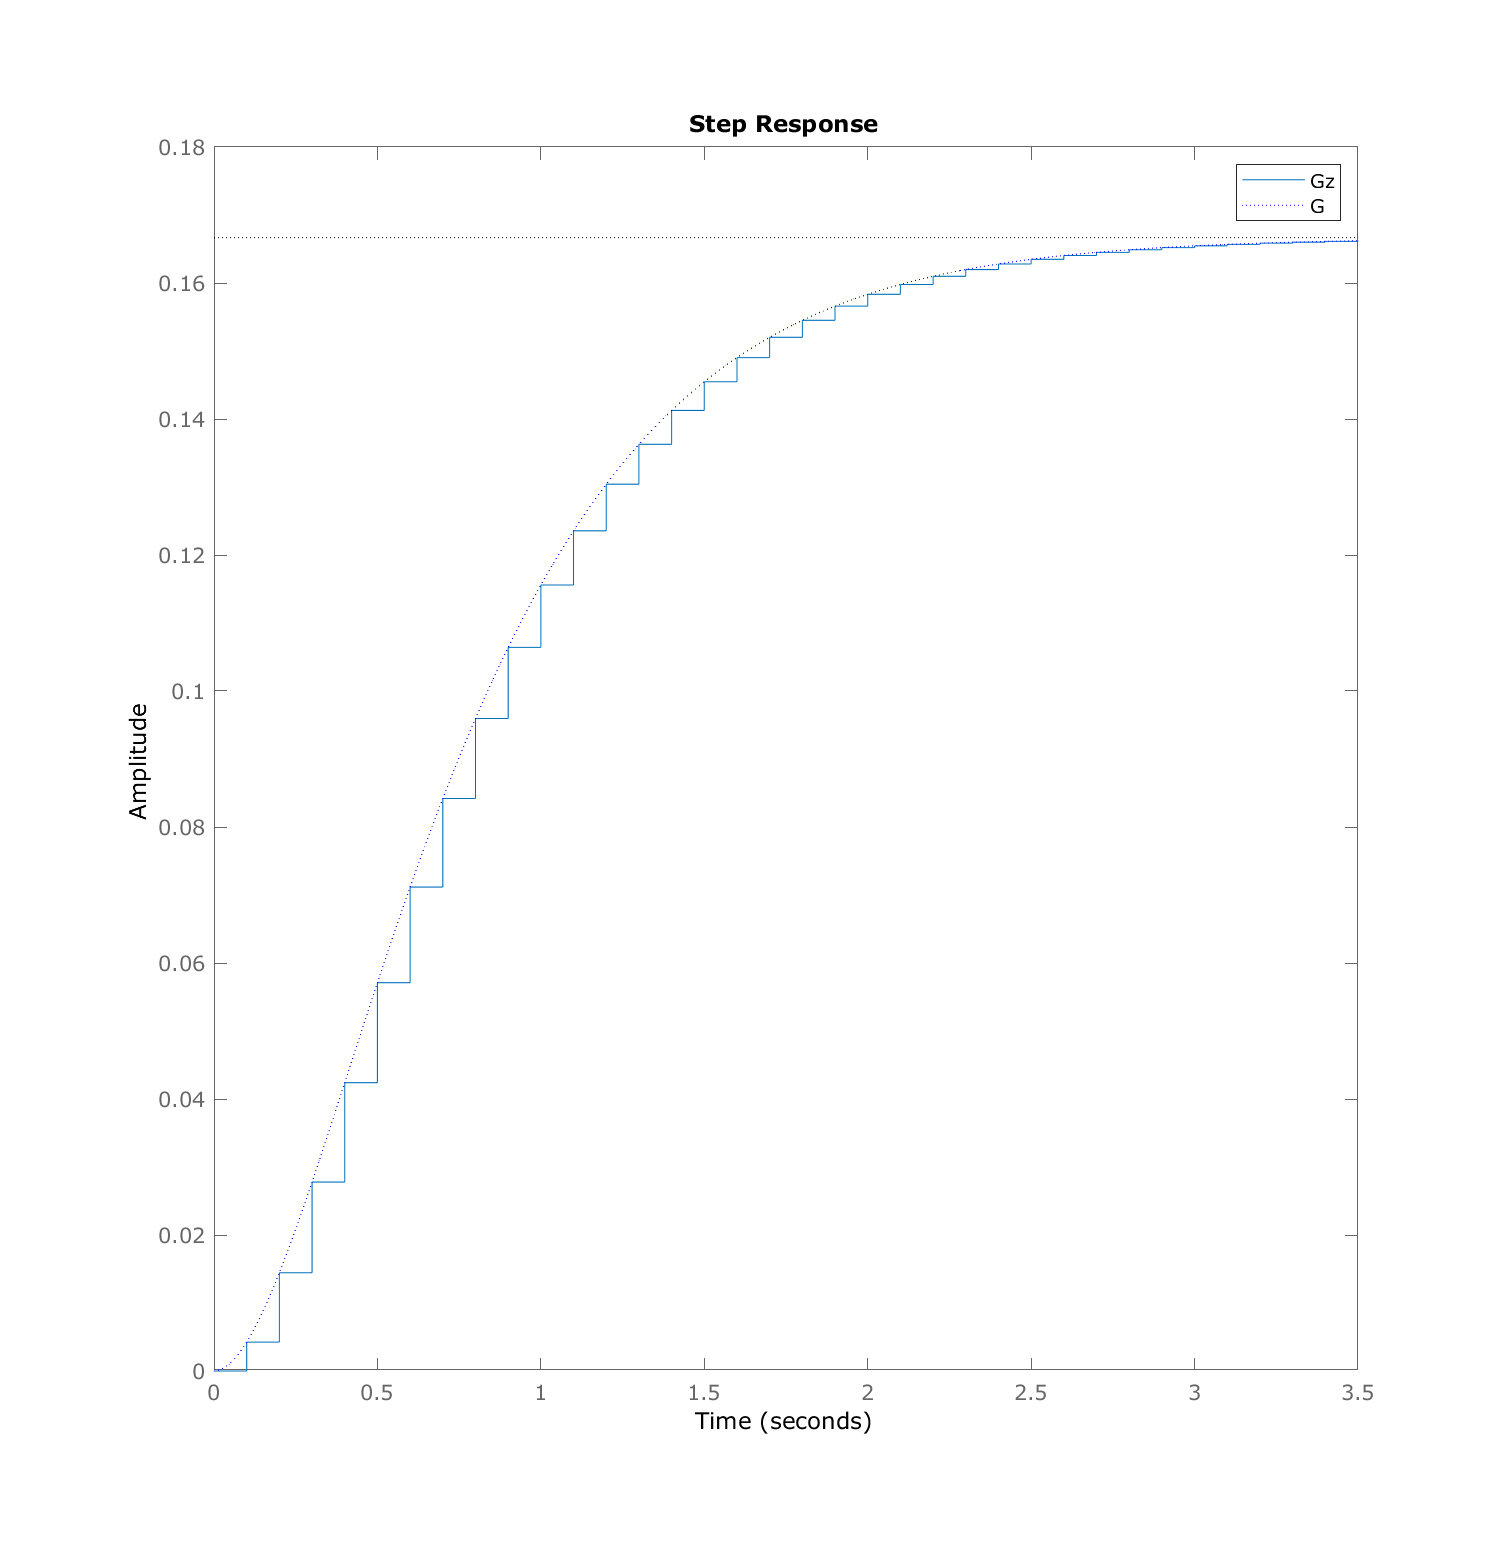
\includegraphics[width=0.8\linewidth]{img/exsim2-plot-g-zoh.png}
    \caption{Resposta ao Degrau Unitário do Sistema Discretizado com um Segurador de Ordem Zero}
\end{figure}

\subsection{Regra Retangular para frente}

Uma outra forma de discretização é por meio de integração numérica. Neste caso basta subsituir $s = \sympy{Gzf}$:

$$
    G_f(z) =  G(z)|_{s = \sympy{Gzf}} = \sympy{Gof}
$$

$$
    G_f(z) = \sympy{simplifyFraction(Gof,z)}
$$

Substituindo o período de amostragem $T=\sympy{nT}$:

\begin{equation}
    G_f(z) = \sympy{Gof.combsimp().subs(T,nT)}
\end{equation}

Neste método o número de polos e zeros é conservado após a discretização, no entanto tráz o problema de que polos estáveis dentro no plano s podem ser mapeados em polos instáveis no plano z a depender do período de amostragem $T$. Quanto menor o período de amostragem maior a chances de termos polos instáveis na realização do sistema discretizado desta forma. Para o período de amostragem $T=\sympy{nT}$  obtemos como resposta ao degrau:

\begin{figure}[H]
    \centering
    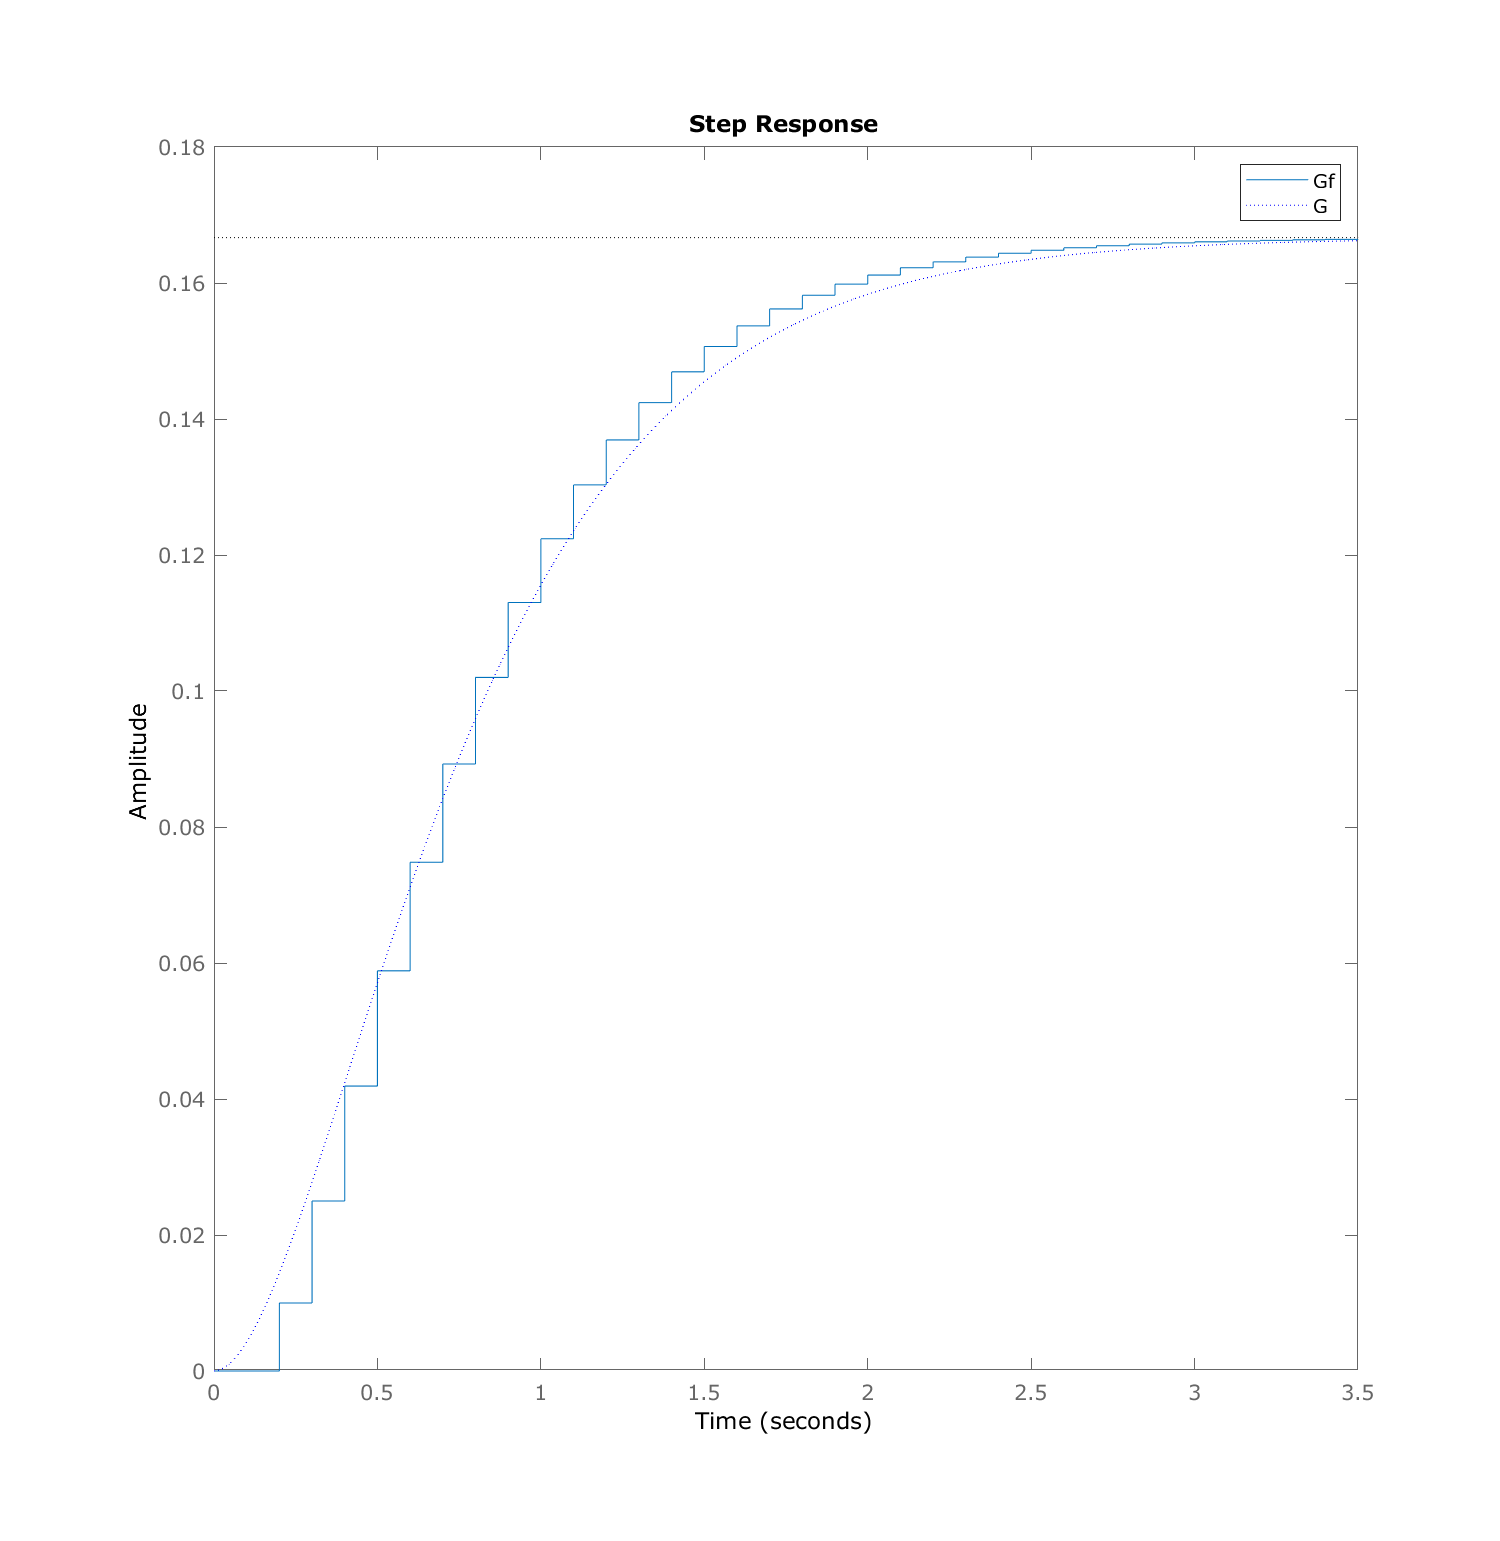
\includegraphics[width=0.8\linewidth]{img/exsim2-plot-g-forward.png}
    \caption{Resposta ao Degrau Unitário do Sistema discretizado pela regra retangular para frente}
\end{figure}

\subsection{Regra Retangular para trás}

Outro método de integração numérica é a Regra Retangular para trás, em que substituimos $s = \sympy{Gzb}$:

$$
    G_b(z) =  G(z)|_{s = \sympy{Gzb}} = \sympy{Gob}
$$

$$
    G_b(z) = \sympy{simplifyFraction(Gob,z)}
$$

Substituindo $T=\sympy{nT}$ temos

\begin{equation}
    G_b(z) = \sympy{Gob.combsimp().subs(T,nT)}
\end{equation}

Com isto é acrescentado um zero a mais na origem para cada polo da função, modificando o comportamento dinâmico do sistema. Do ponto de vista de estabilidade o problema é que polos instáveis no plano s podem vir a ser mapeados como estáveis em z. Desta forma somente a análise do sistema em no plano z pode não representar adequadamente o perfil de estabilidade no plano s do sistema.

\begin{figure}[H]
    \centering
    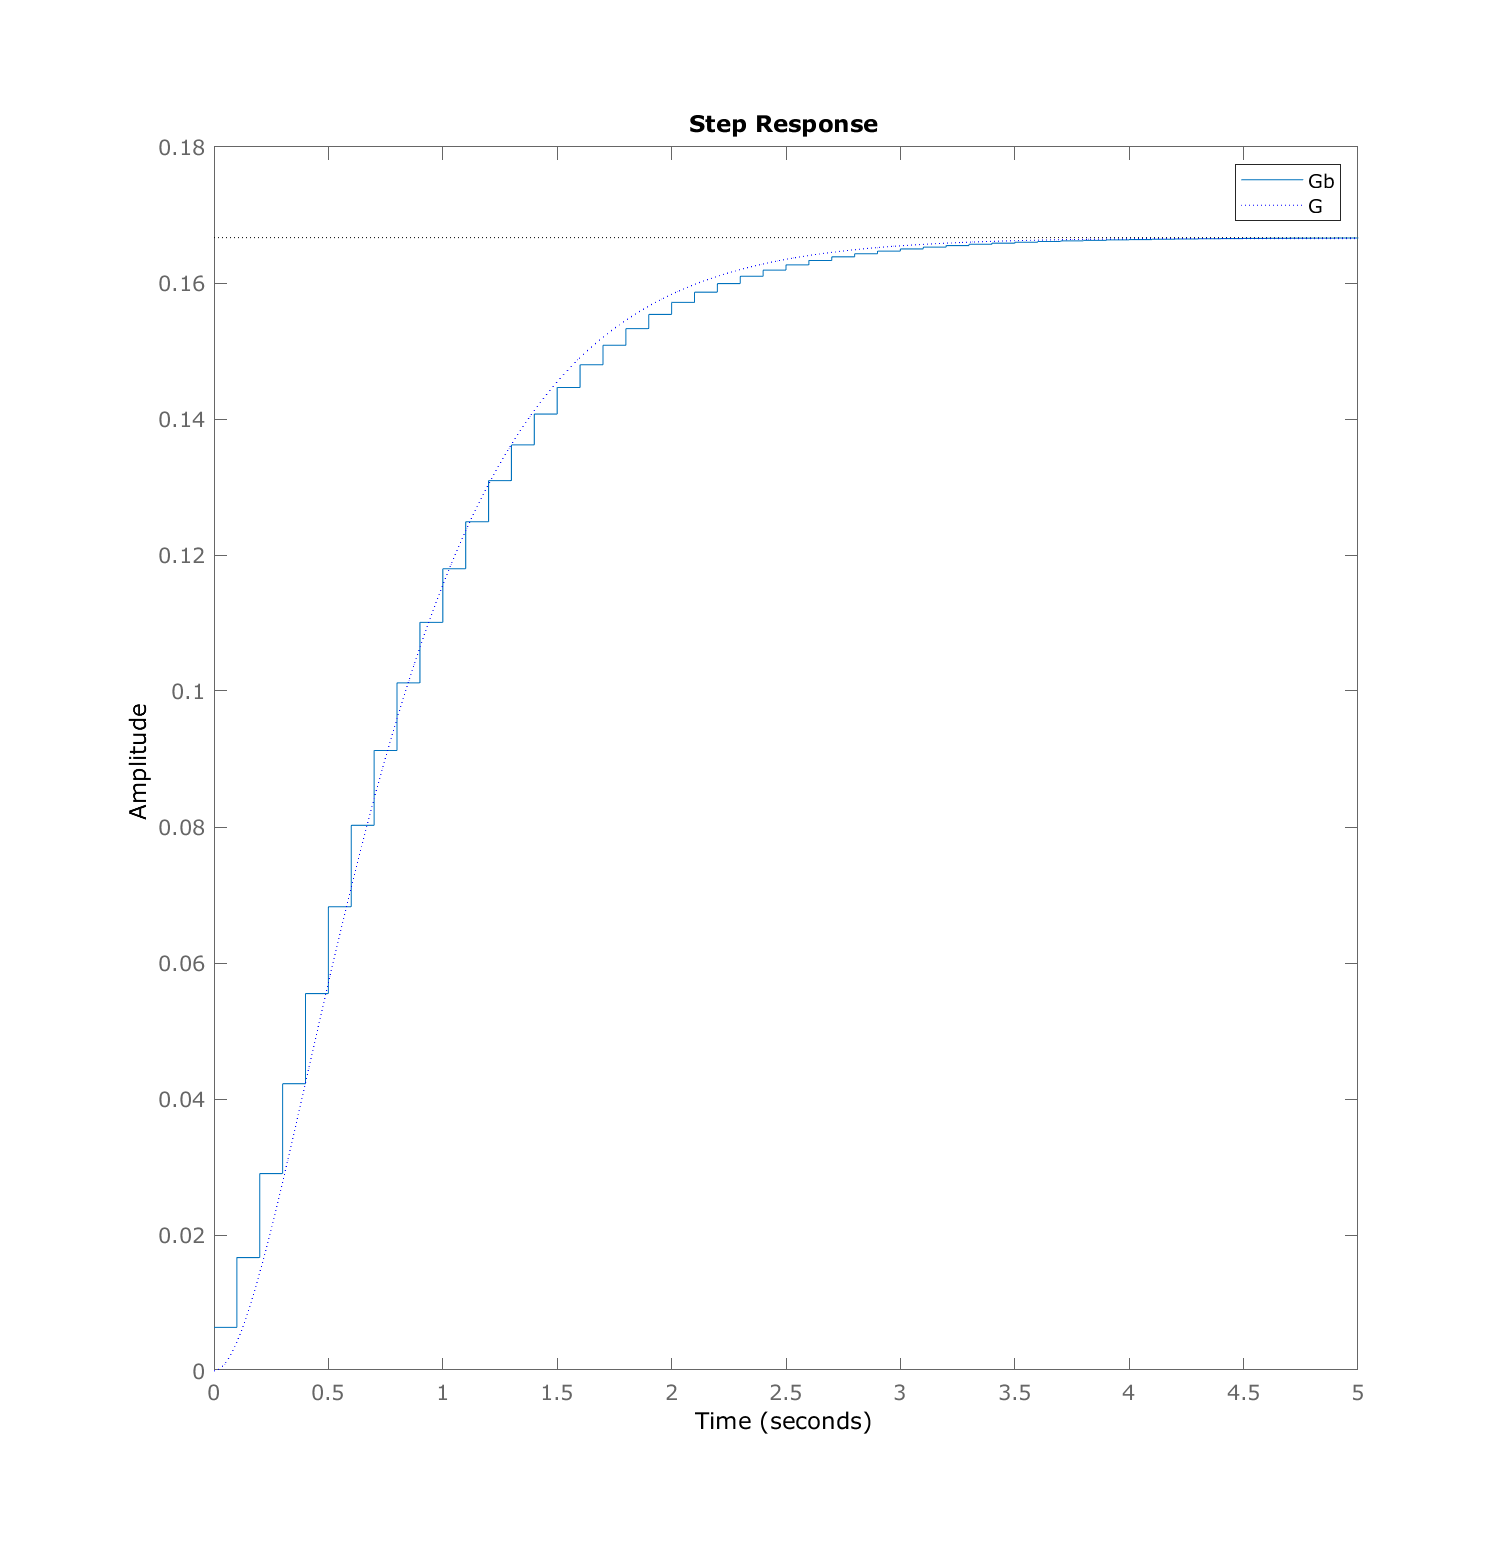
\includegraphics[width=0.8\linewidth]{img/exsim2-plot-g-backward.png}
    \caption{Resposta ao Degrau Unitário do Sistema discretizado pela regra retangular para trás}
\end{figure}

\subsection{Regra trapezoidal}

$$
    G_d(z) =  G(z)|_{s = \sympy{Gzd}} = \sympy{God}
$$

$$
    G_d(z) = \sympy{simplifyFraction(God,z)}
$$

Em particular para $T=\sympy{nT}$ temos

\begin{equation}
    G_d(z) = \sympy{God.combsimp().subs(T,nT)}
\end{equation}

Neste caso, é acrescentado um zero a mais e 1 para cada polo existente. Dos métodos de discretização por integração avaliados foi o que mais aproximou o comportamento do sistema para uma mesma taxa de amostragem. Em termos de estabilidade, permite que o mapeamento completo do semi plano direito s dentro do circulo unitário no plano z. Desta forma 

\begin{figure}[H]
    \centering
    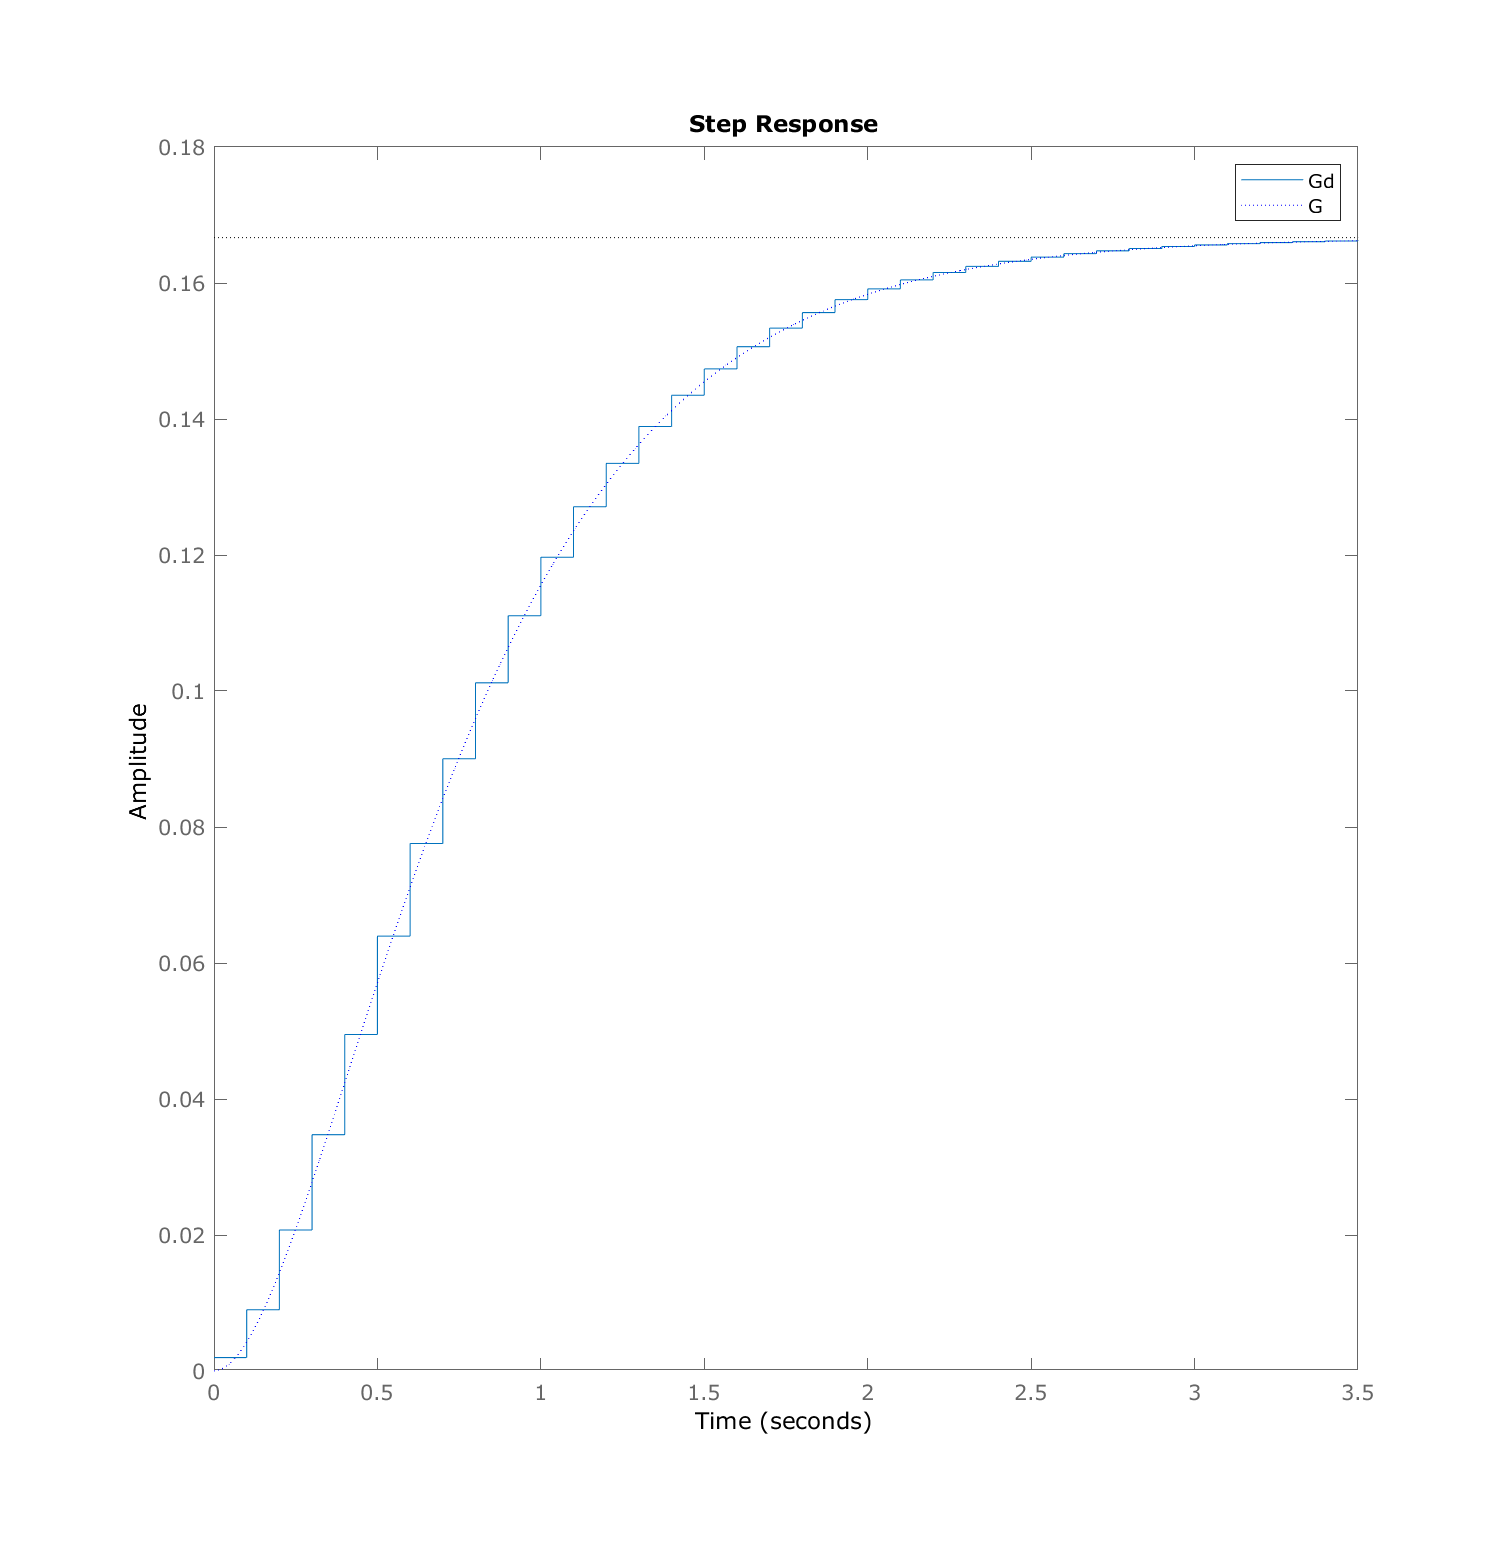
\includegraphics[width=0.8\linewidth]{img/exsim2-plot-g-trap.png}
    \caption{Resposta ao Degrau Unitário do Sistema discretizado pela regra trapezoidal}
\end{figure}

Um aspecto interessante percebido na simulação e resultado da forma de construção deste método de integração que que a função discretizada possui o mesmo valor do sistema continuo na metade do período de amostragem. isto é $G_d(kT+T/2) = G(kT+T/2$ para todo $k$.

\subsection{Mapeamento exato de pólos e zeros}

A função de transferência têm como polos $s_1=-2$ e $s_2=-3$. Mapeando no plano z temos $z = e^{sT}$

Este método possui as mesmas propriedades quanto a estabilidade que o método de integração pela Regra Trapezoidal, no entanto computacionalmente é mais caro de ser utilizado.

\begin{figure}[H]
    \centering
    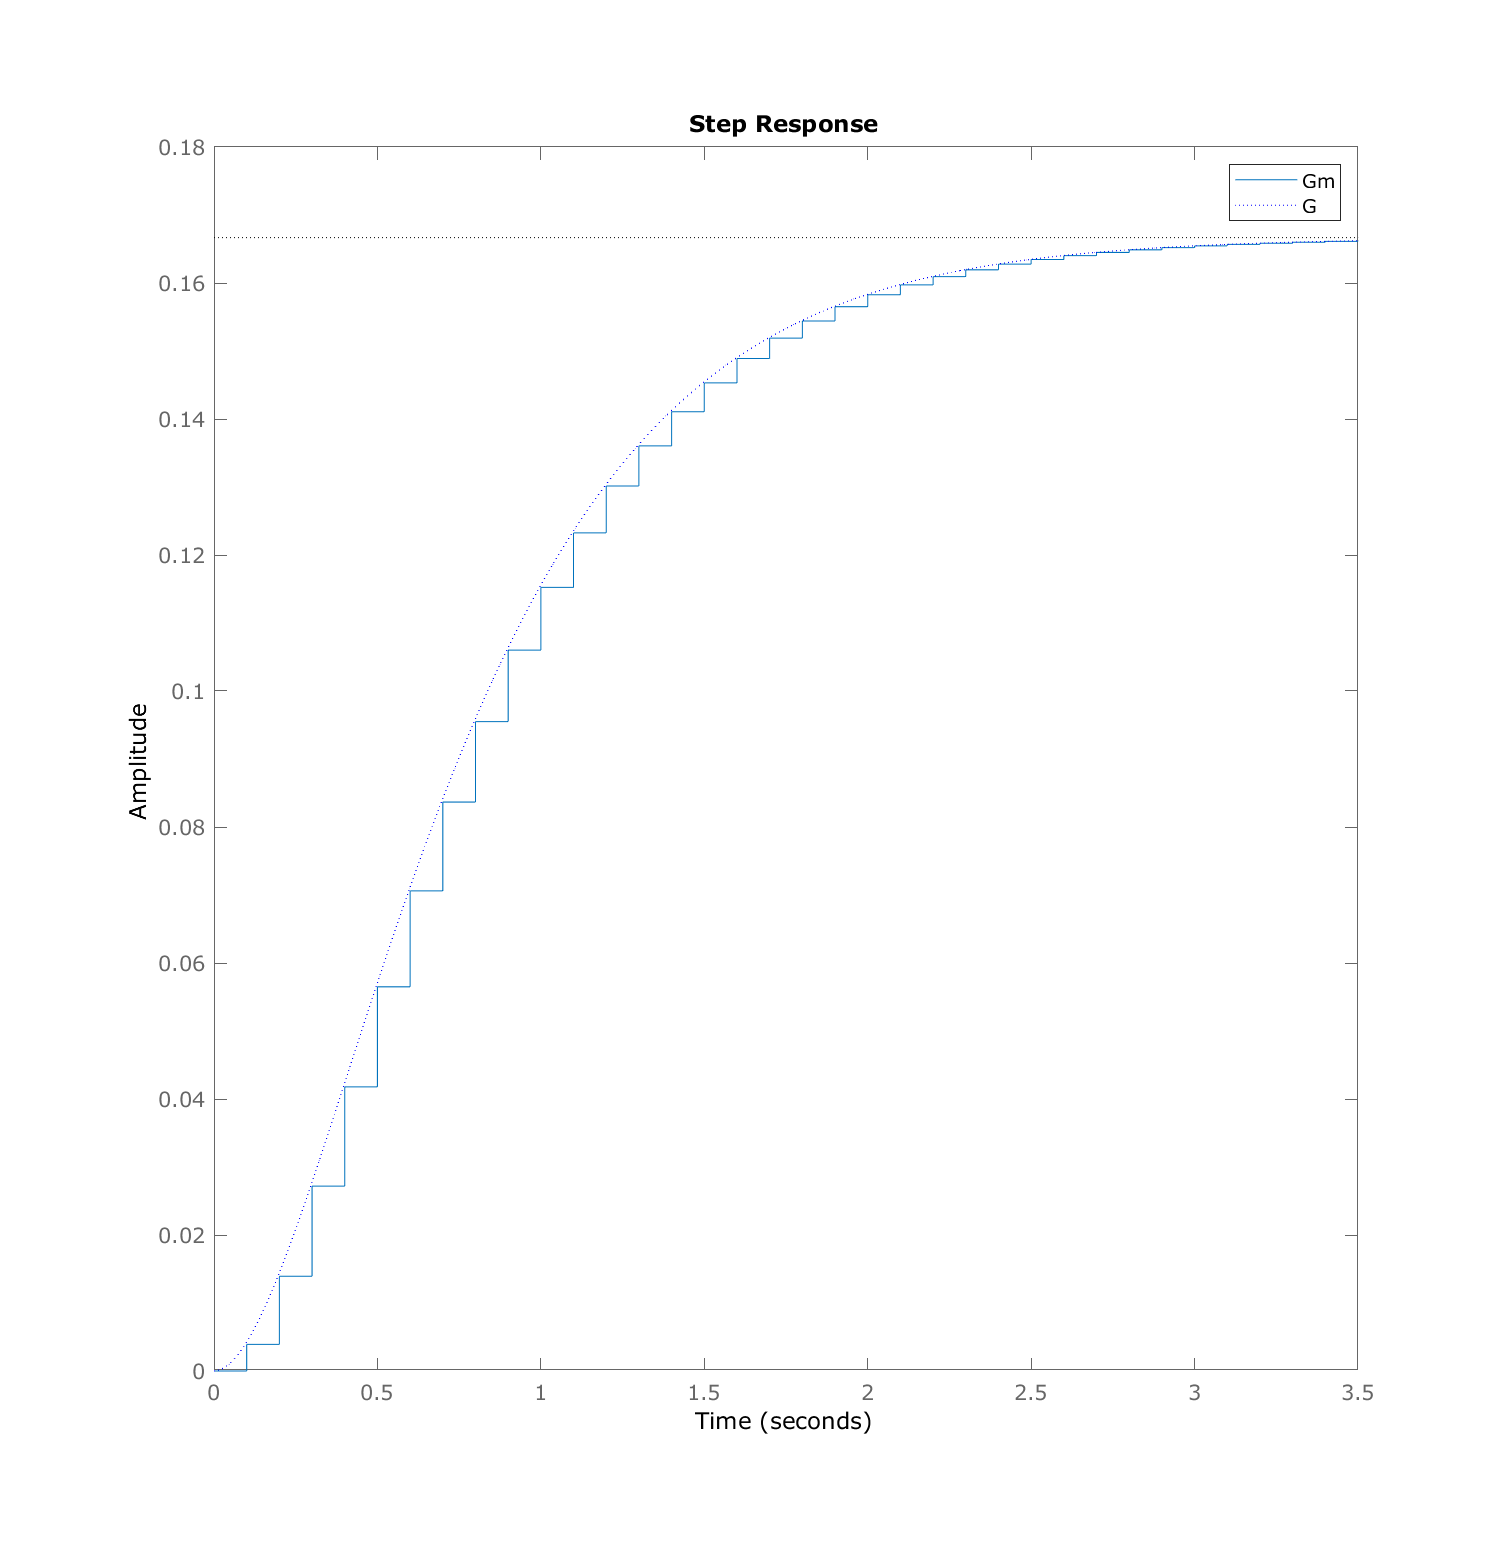
\includegraphics[width=0.8\linewidth]{img/exsim2-plot-g-matched.png}
    \caption{Resposta ao Degrau Unitário do Sistema discretizado pela regra trapezoidal}
\end{figure}

Pela simulação temos o sistema discretizado possui exatamente o mesmo valor que o sistema contínuo em todos os instantes de $t$.


\begin{figure}[H]
    \centering
    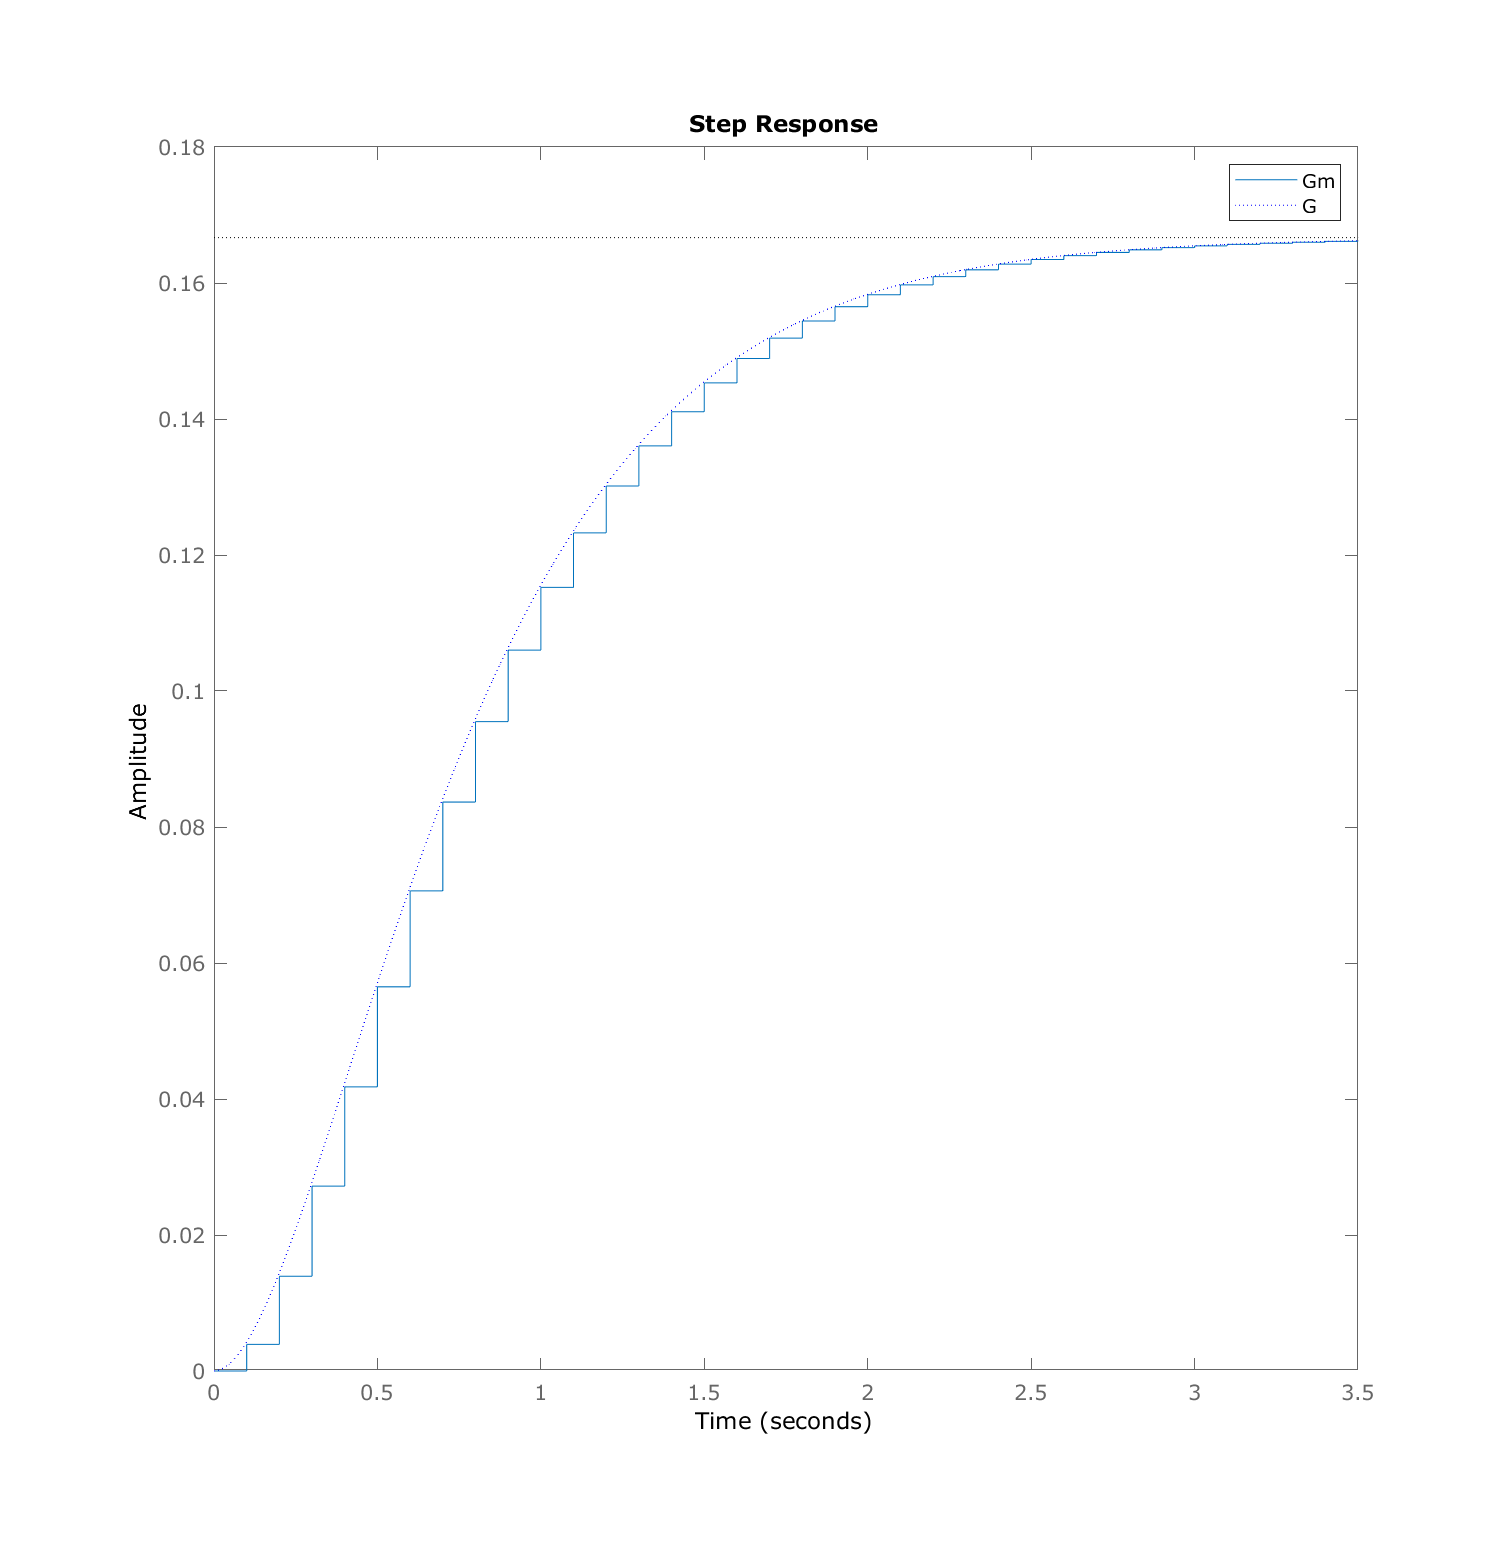
\includegraphics[width=0.8\linewidth]{img/exsim2-plot-g-matched.png}
    \caption{Resposta ao Degrau Unitário do Sistema discretizado por mapeamento exato dos polos}
\end{figure}

\section{Projeto Sistema em Tempo Discreto}

\subsection{Sistema em Malha Fechada}

Dado $G(s)$

\begin{equation}
    G(s) = \frac{Y(s)}{U(s)} \sympy{G2}
\end{equation}

\begin{equation}
    U(s) = \sympy{G1}U_C(s) - \sympy{H2}Y(s)
\end{equation}

Aplicando o sinal de controle e fechando a malha obtemos:

$$G_{mf}(s) = \frac{Y(s)}{U_c(s)} = \sympy{G2mf}$$

Substituindo $a = \sympy{2*w0}$ e $b = \sympy{w0/2}$ temos

$$
G_{mf}(s) = \sympy{G2mf.subs([(a,2*w0),(b,w0/2)])}
$$
$$
G_{mf}(s) = \sympy{G2mf.subs([(a,2*w0),(b,w0/2),(kc,2*J*w0*w0/kp)])}
$$

Simplificando

\begin{equation}
    G_{mf}(s) = \sympy{simplifyFraction(G2mf.subs([(a,2*w0),(b,w0/2),(kc,2*J*w0*w0/kp)]),s)}
\end{equation}

\subsection{Resposta em frequência}

\begin{figure}[H]
    \centering
    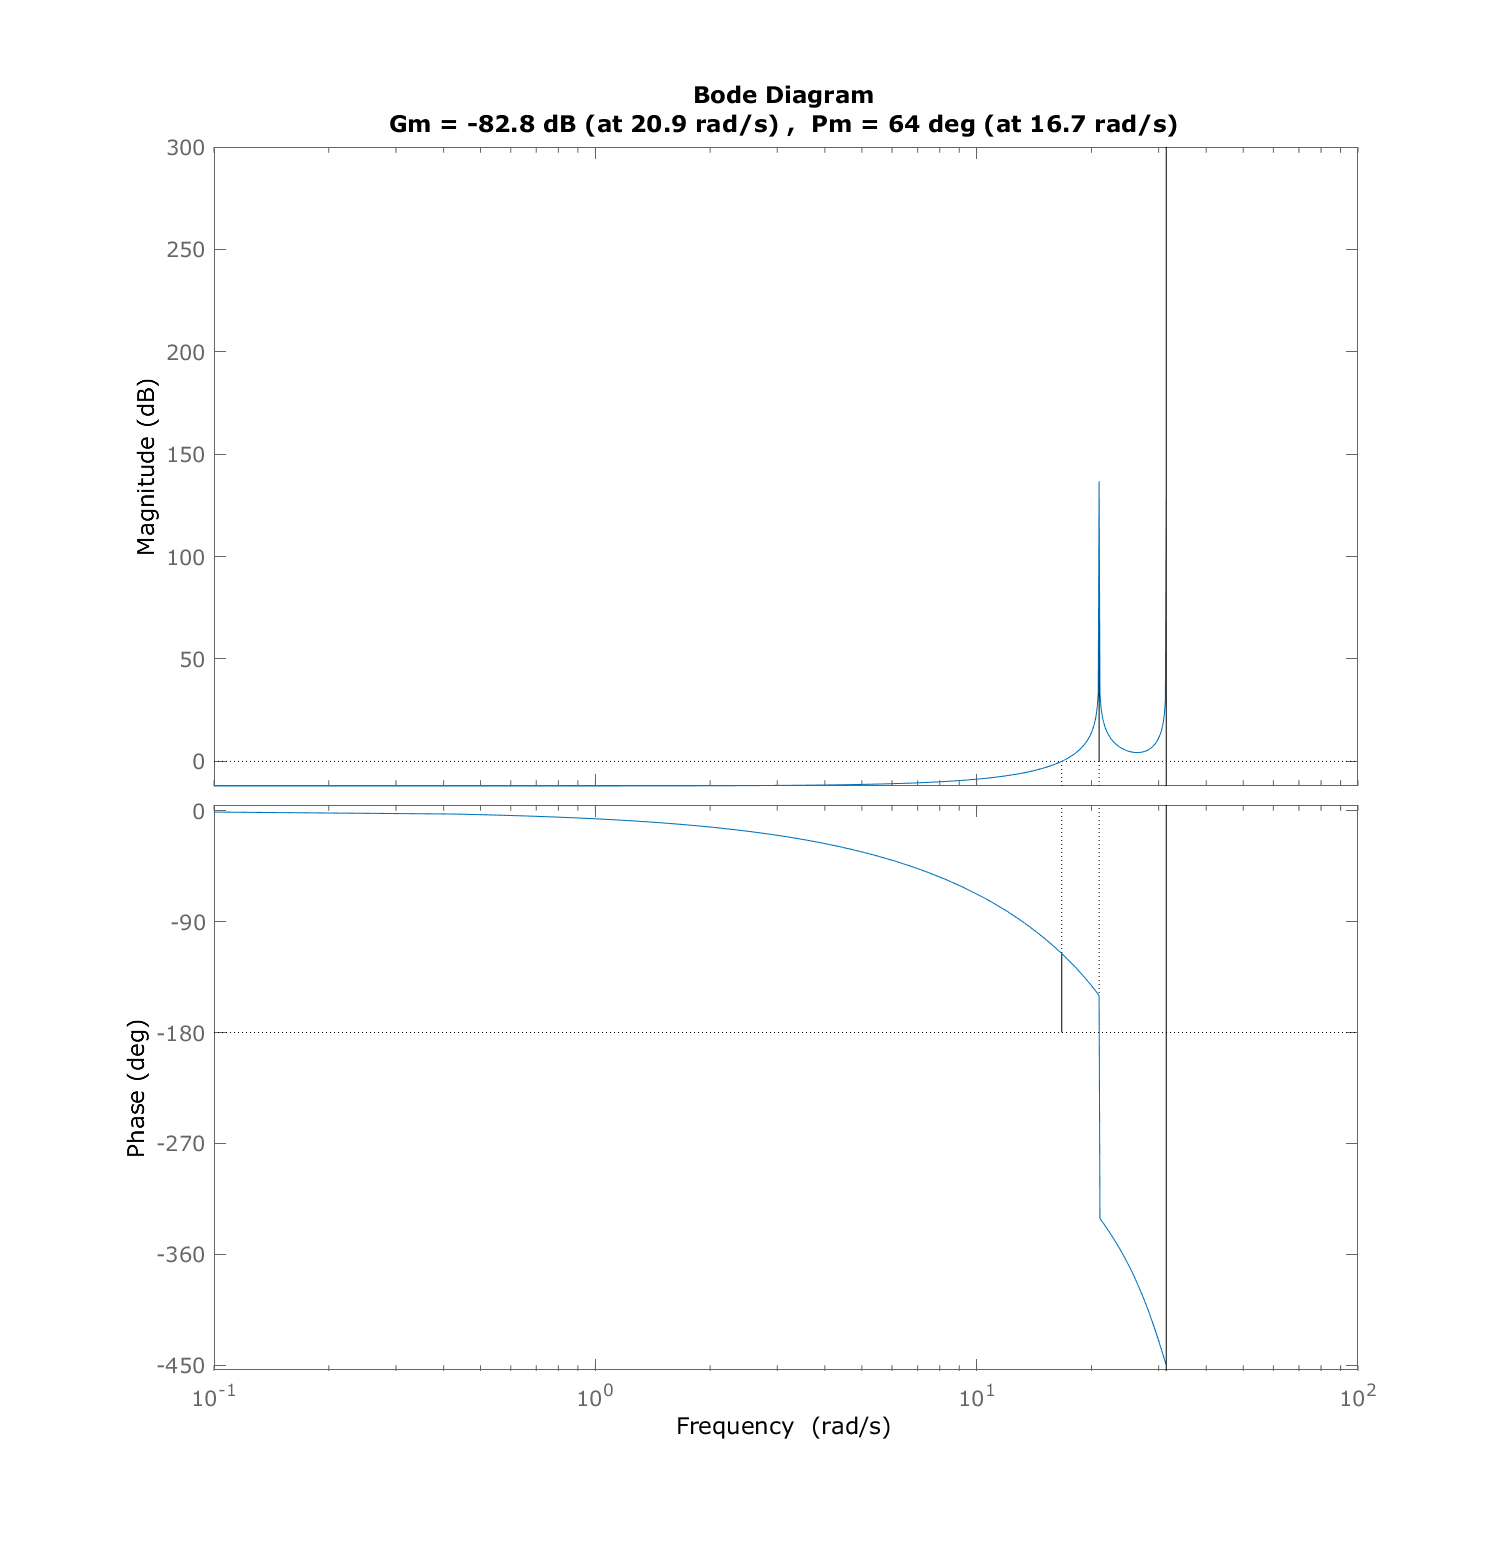
\includegraphics[width=0.9\linewidth]{img/exsim2-plot-bode2.png}
    \caption{Diagrama de bode do sistema ($w_0=1$)}
\end{figure}

\subsection{Ação de Controle}

Dado seguinte expressão da ação de controle:
$$U(s) = \sympy{G1}U_C(s) - \sympy{H2}Y(s)$$

Podemos reescrever como:
$$U(s) = kc\left( \frac{b}{a}U_C(s) - \frac{(s+b-a+a)}{s+a}Y(s) \right)$$
$$U(s) = kc\left( \frac{b}{a}U_C(s) - \frac{(s+a)}{s+a}Y(s) - \frac{(b-a)}{s+a}Y(s) \right)$$
$$U(s) = kc\left( \frac{b}{a}U_C(s) - Y(s) + \frac{(a-b)}{s+a}Y(s) \right)$$

Por fim temos
\begin{equation}
    U(s) = kc\left( \frac{b}{a}U_C(s) - Y(s) + \frac{(a-b)}{(s+a)}Y(s) \right)
\end{equation}

\subsection{Simulink}

\begin{figure}[H]
    \centering
    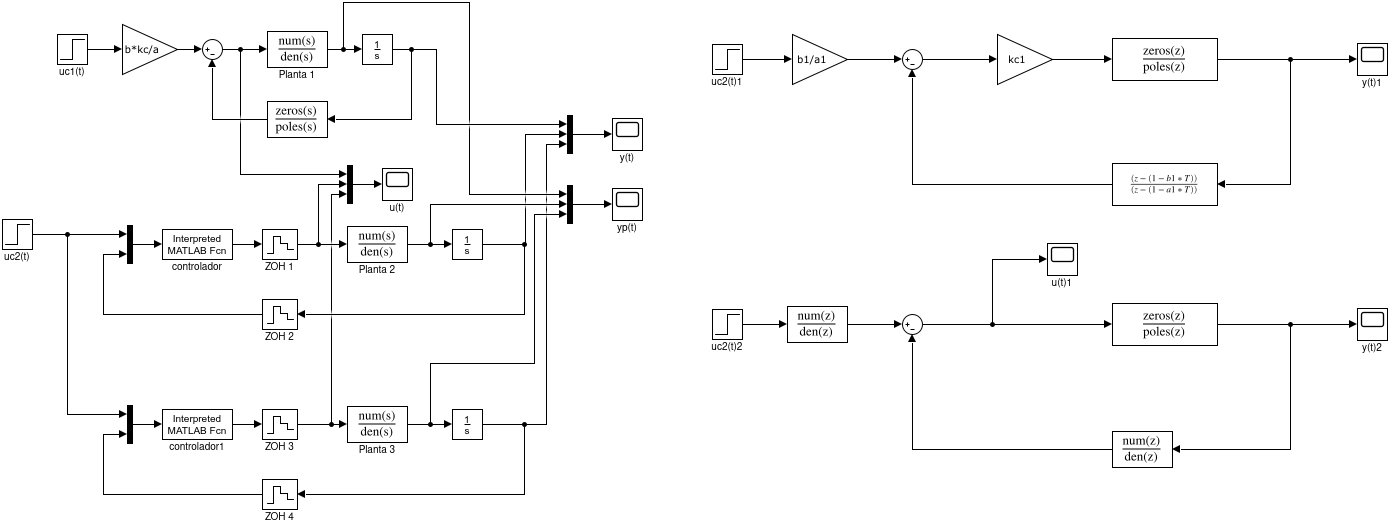
\includegraphics[width=0.8\linewidth]{img/exsim2model.png}
    \caption{Diagrama de Blocos do Sistema no Simulink}
    \label{fig:ex2-simulink}
\end{figure}

\subsubsection{Simulação}

Simulando o sistema da figura \ref{fig:ex2-simulink} para os períodos $T=0.2s$ , $T=0.5s$ e $T=1.08s$ 

\begin{figure}[H]
    \centering
    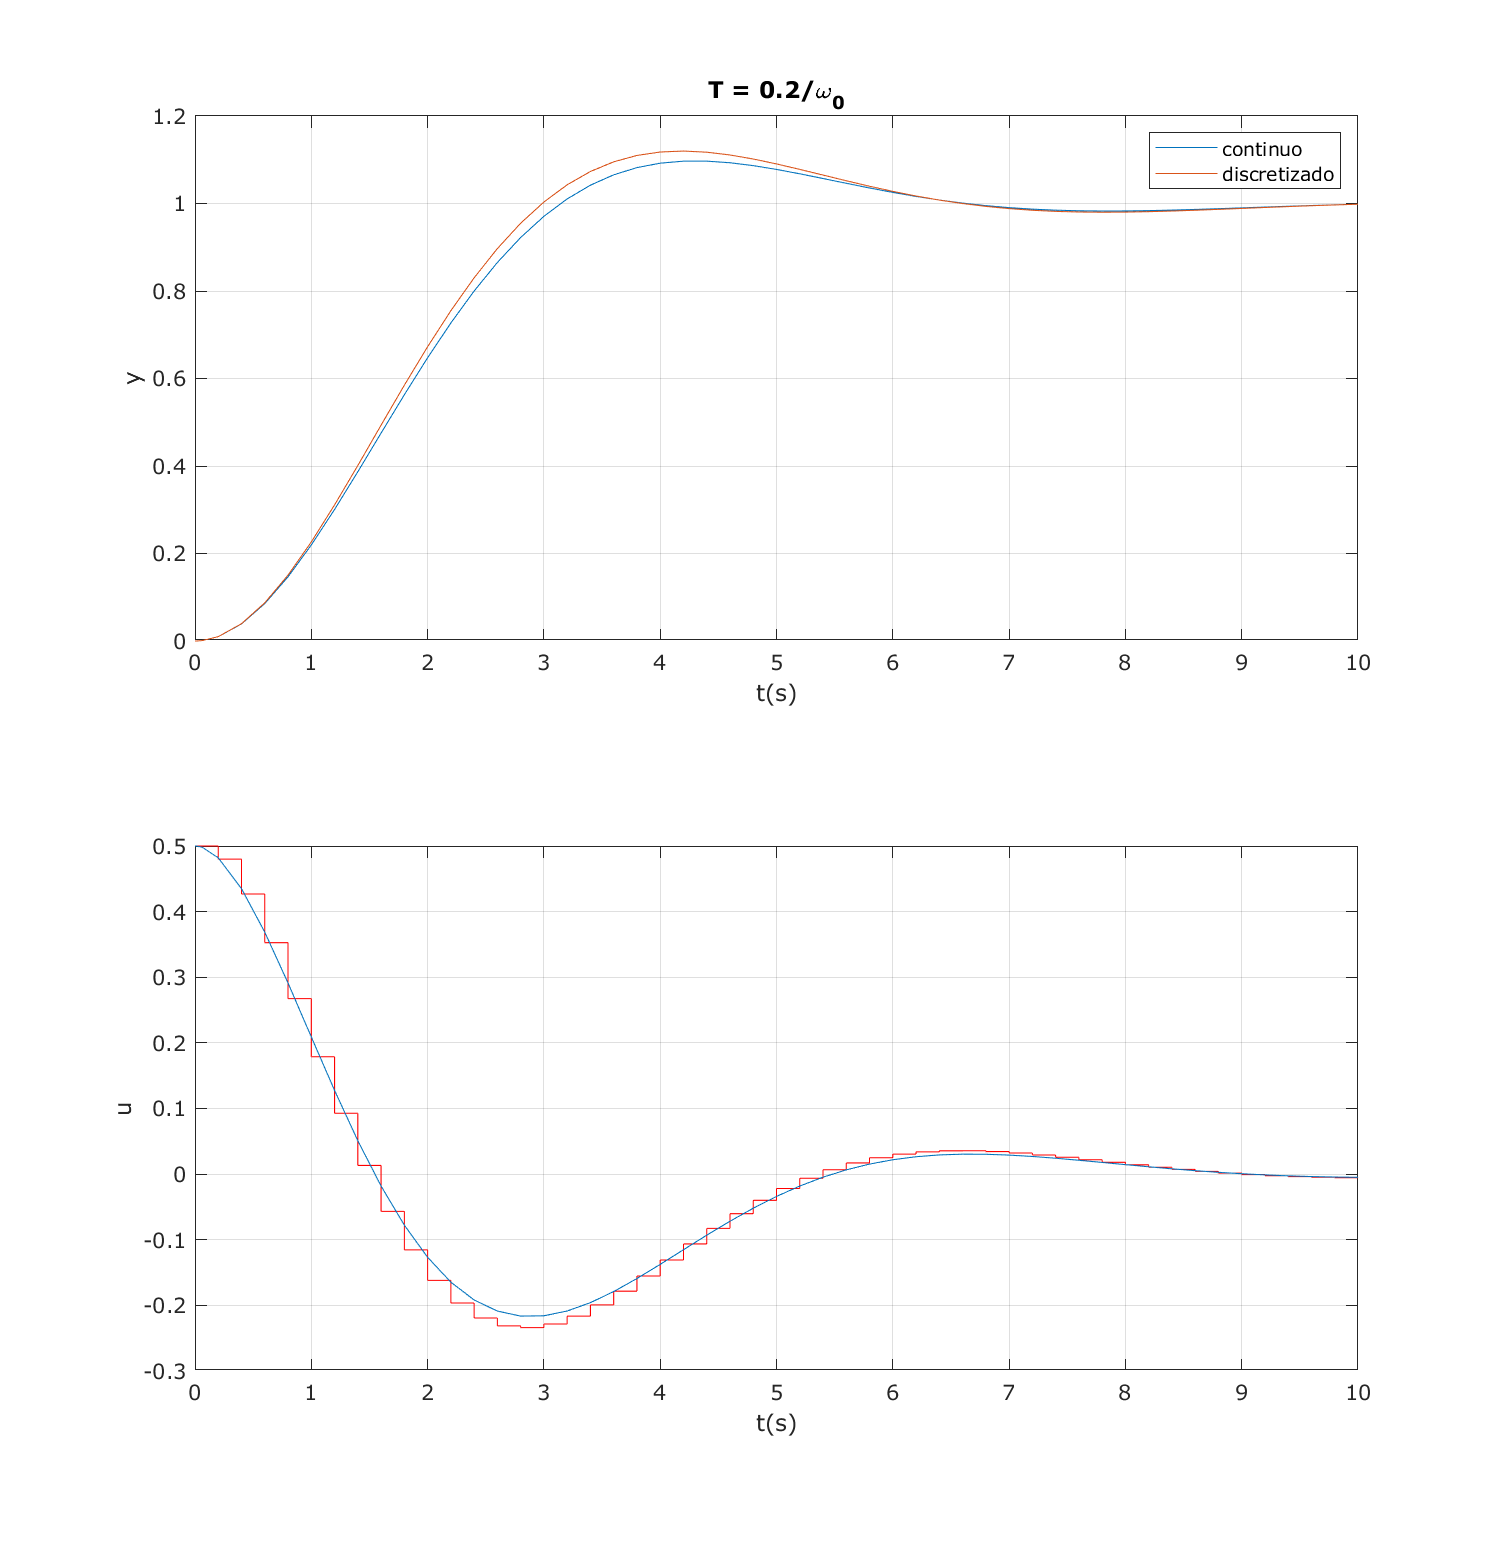
\includegraphics[width=0.9\linewidth]{img/exsim2-plot-sim-t02.png}
    \caption{Resposta Simulação $T=0.2s$}
\end{figure}

\begin{figure}[H]
    \centering
    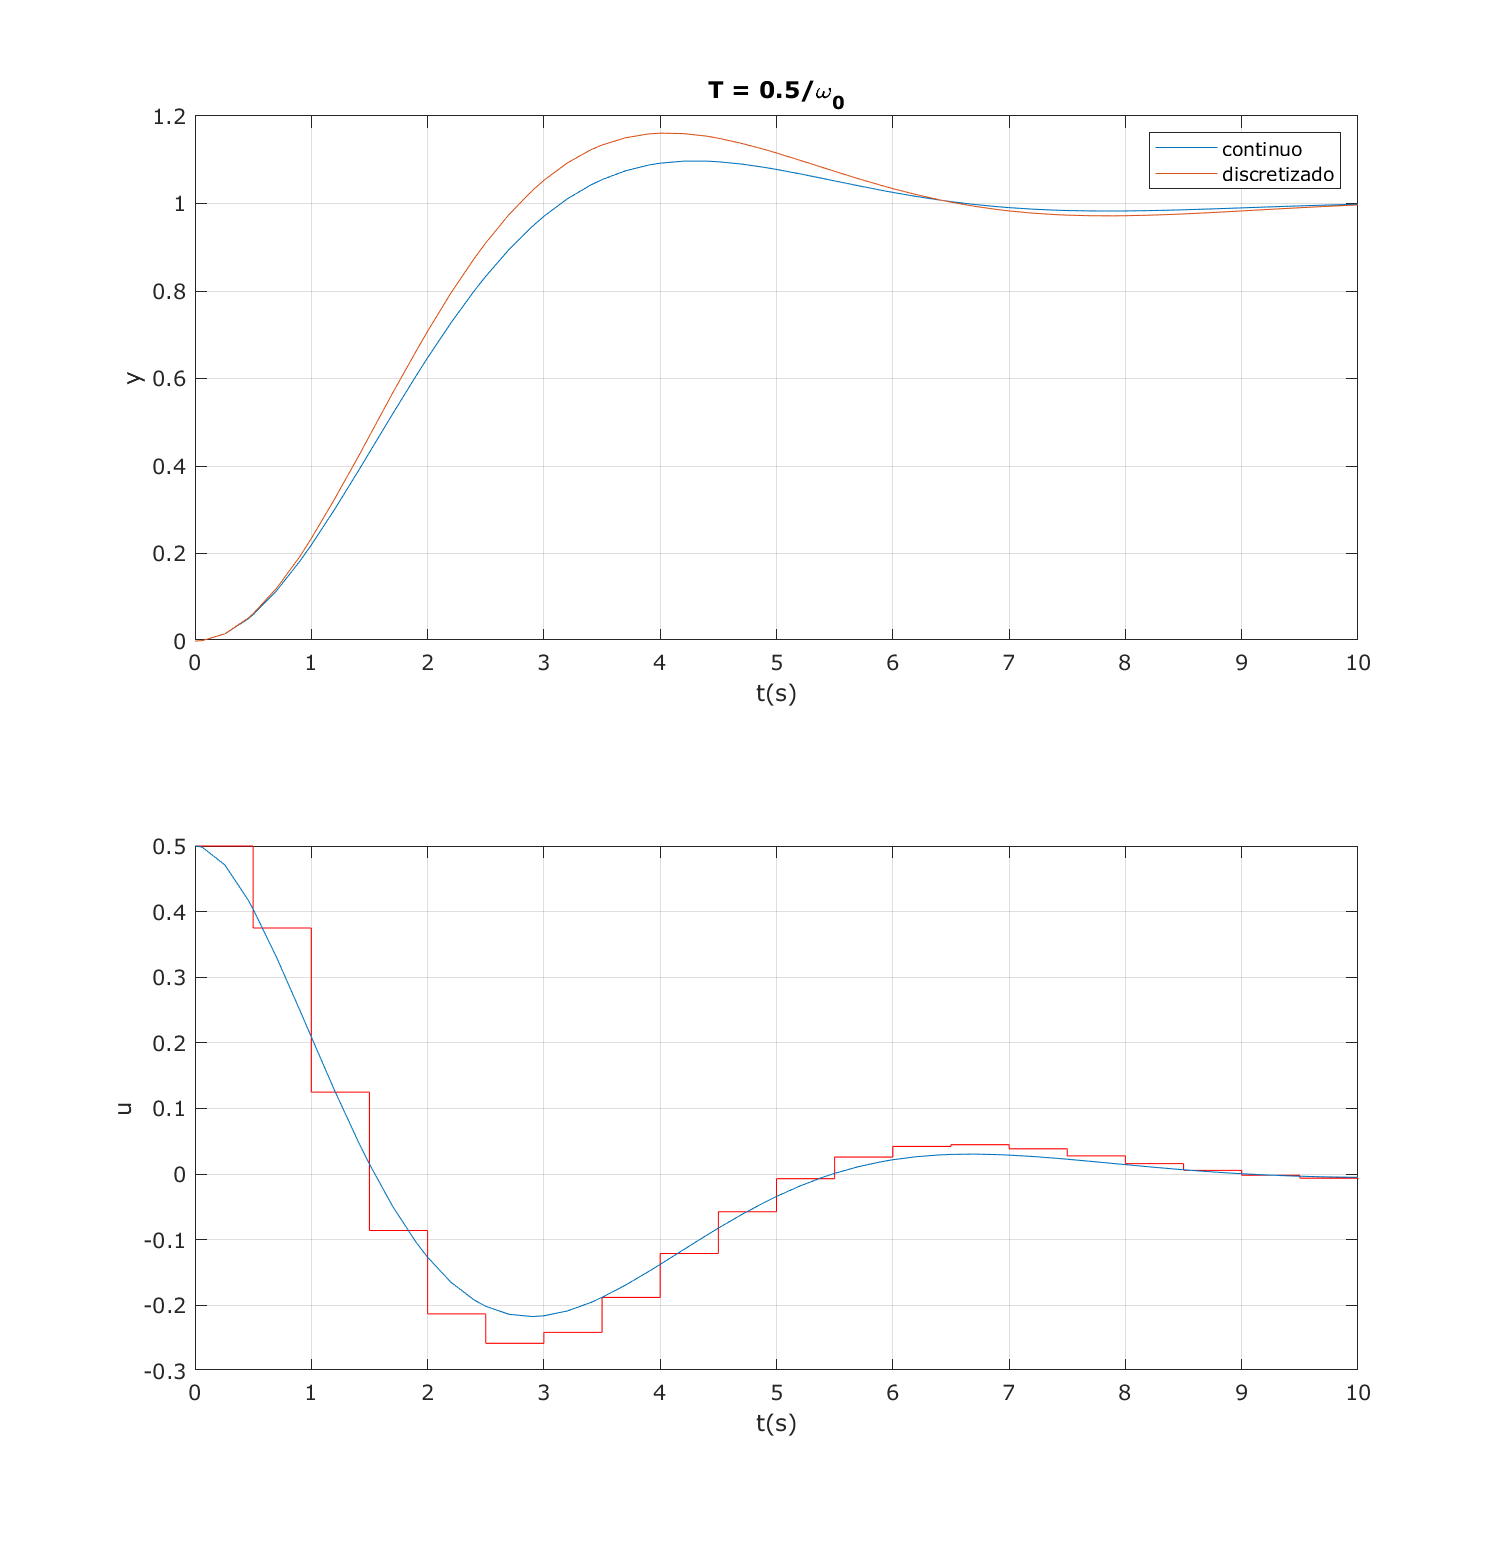
\includegraphics[width=0.9\linewidth]{img/exsim2-plot-sim-t05.png}
    \caption{Resposta Simulação $T=0.5s$}
\end{figure}

No entanto para $t=1.08s$ observamos que o sistema ficou instável. Conforme comentado, para sistemas discretizados o aumento do período de amostragem pode implicar na instabilidade da realização do sistema discretizado.

\begin{figure}[H]
    \centering
    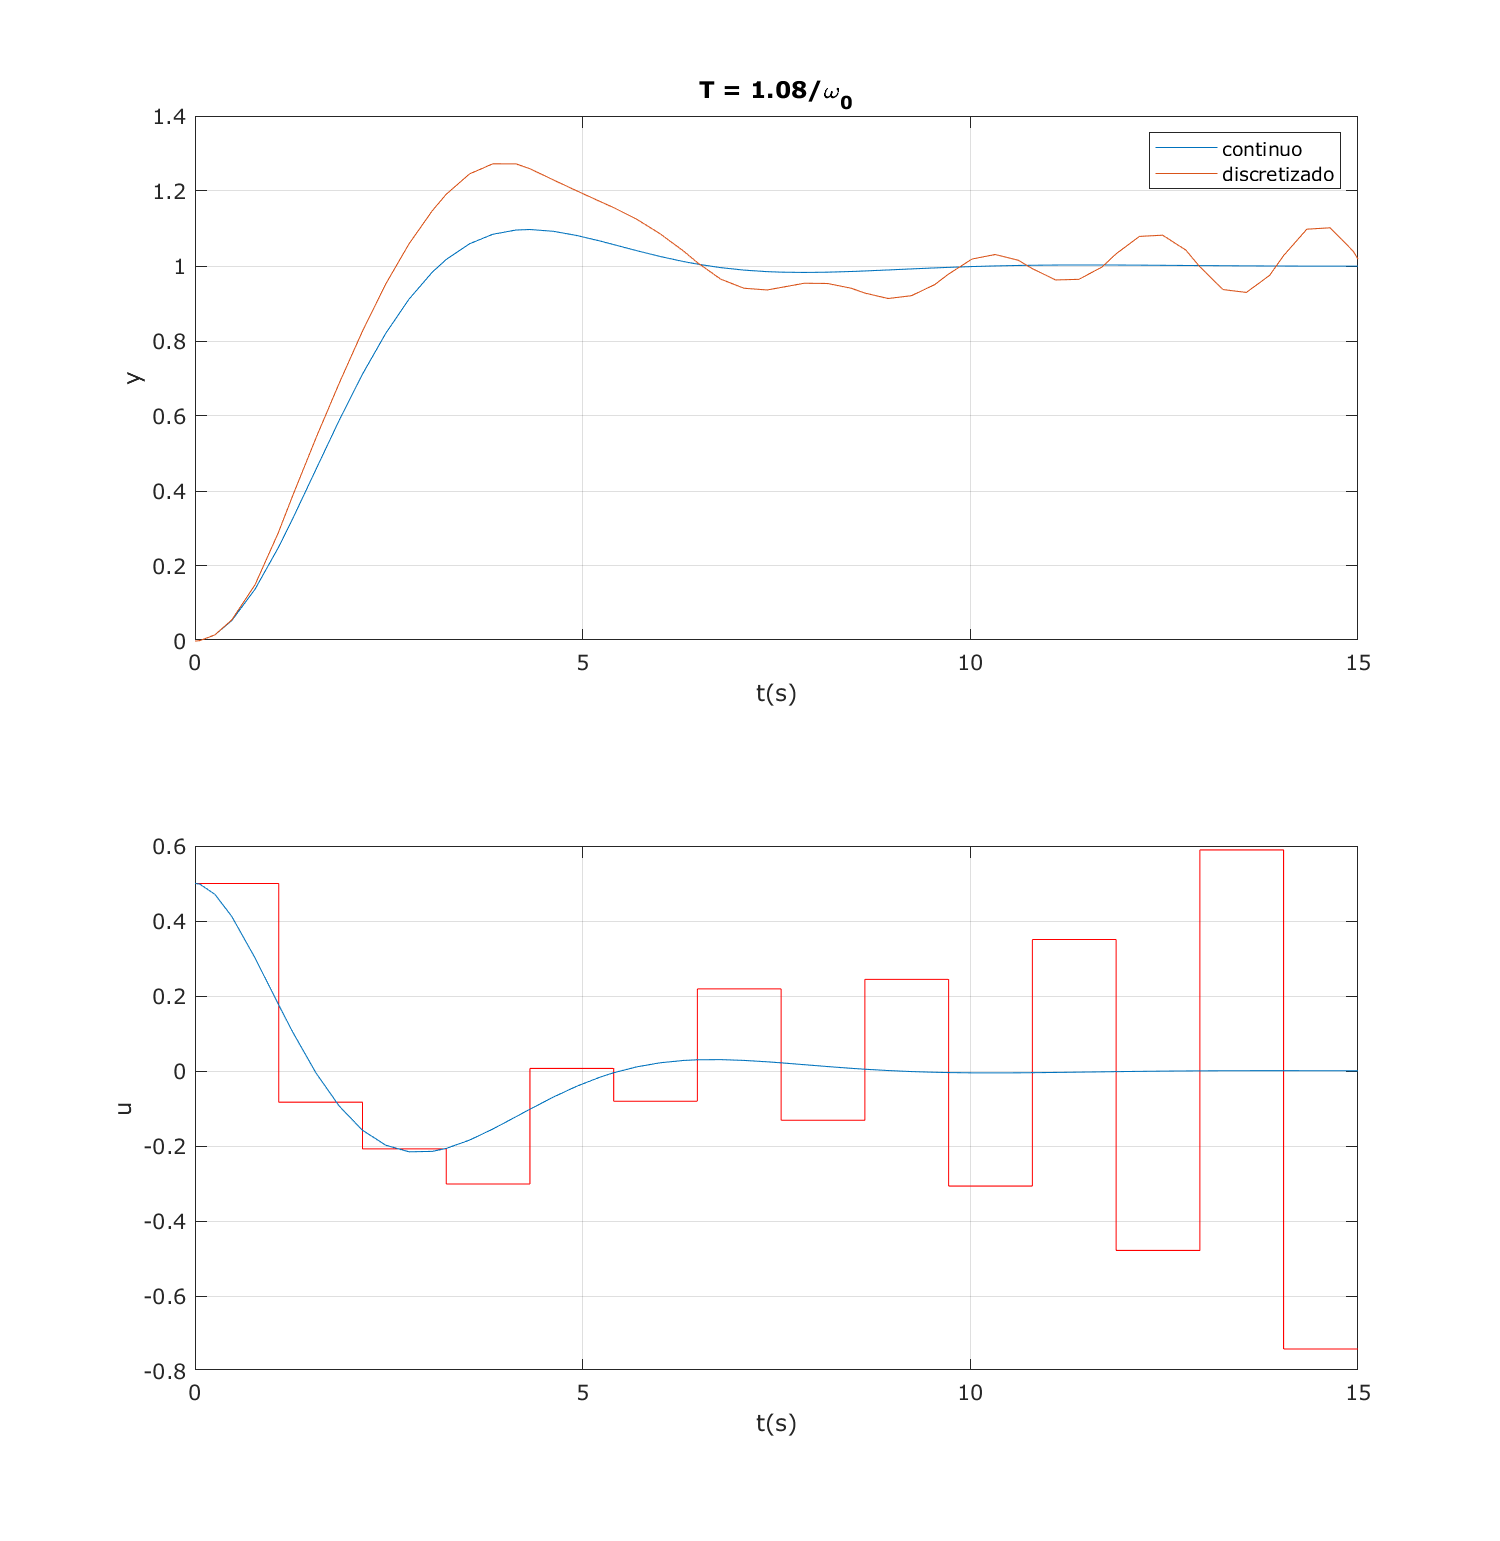
\includegraphics[width=0.9\linewidth]{img/exsim2-plot-sim-t108.png}
    \caption{Resposta Simulação $T=1.08s$}
\end{figure}

%%\section{Conclusão}

% ------------------------------------------------------------------------------

% Referências
\addcontentsline{toc}{section}{Referências} % Adiciona linha no indice
\bibliographystyle{abbrv} % Define Estilo e gera bibliografia
\bibliography{references} % Adiciona Arquivo com Referências

% Acrescentadas no arquivo references.bib
% para usa-las no texto basta usar \citep{}
% para citar sem usar no texto basta usar \nocite{}
\nocite{sympy}
\nocite{pythontex}
\nocite{matlabcontrol}
\nocite{matlabsymbolic}

% ------------------------------------------------------------------------------
\newpage
\section*{Anexos}
\addcontentsline{toc}{section}{Anexos} % Adiciona linha no indice
\subsection*{Python}

Com exceção da transformada z, para os cálculos e demonstrações foi utilizado o pacote \textit{Python}\TeX\ \cite{pythontex} para o \LaTeX\ em conjunto da bibliteca \textit{sympy}\cite{sympy}. Segue o script completo em python:

\inputminted[xleftmargin=15pt,linenos,frame=single,framesep=5pt]{python}{../python/exsim2.py}

\newpage
\subsection*{Matlab}

\subsubsection*{Parte 1}
Para o desenho dos gráficos e simulações foi utilizado o \textit{Matlab} em conjunto das toolbox \textit{Control System}\cite{matlabcontrol} e \textit{Symbolic Math}\cite{matlabsymbolic}. Segue o código referente usado

\inputminted[xleftmargin=15pt,linenos,frame=single,framesep=5pt]{matlab}{../matlab/exsim2/exsim2.m}

\subsubsection*{Parte 2}
Na segunda parte foi utilizado uma versão modificada do script em \textit{Matlab} fornecido pelo professor:
\inputminted[xleftmargin=15pt,linenos,frame=single,framesep=5pt]{matlab}{../matlab/exsim2/exsim2script.m}



% ------------------------------------------------------------------------------
\end{document}
